\subsection{Norms and traces of integers}

PROPOSITION 17. Let A be a ring, B a (commutative) A-algebra and X a square matrix of order n over B; the following properties are equivalent:

\begin{enumerate}
\def\labelenumi{(\alph{enumi})}
\item
  \(X\) is integral over A.
\item
  There exists a finitely generated sub-A-module \(\mathbf{M}\) of \(\mathbf{B}^n\) such that \(X.x\in \mathbf{M}\) for all \(x\in \mathbf{M}\) and \(\mathbf{M}\) is a system of generators of the B-module \(\mathbf{B}^n\) .
\item
  The coefficients of the characteristic polynomial of \(X\) are integral over \(\mathbf{A}\) .
\end{enumerate}

  If \(\chi(T) = \det(T.1 - X)\) is the characteristic polynomial of \(X\) , the Cayley-Hamilton Theorem shows that \(\chi(X) = 0\) (Algebra, Chapter VII, § 5, no. 4, Remark 1) and, as \(\chi\) is a monic polynomial, (c) implies (a) by no. 1, Proposition 6.

  Suppose in the second place that (a) holds. If \((e_i)_{1 \leqslant i \leqslant n}\) is the canonical basis of \(B^n\) , the sub-A-module M of B generated by the \(X^k \cdot e_i\) ( \(1 \leqslant i \leqslant n, k \geqslant 0\) ) is a finitely generated A-module, since the A-algebra A[X] is a finitely generated A-module (no. 1, Theorem 1); as M contains the \(e_i\) , it is seen that (a) implies (b); the converse is a consequence of no. 1, Theorem 1, condition \((E_{\mathrm{III}})\) .

  Finally let us prove that (a) implies (c); as X is integral over A and a fortiori over the polynomial ring A[T], T.1 - X is also integral over A[T] and by no. 3, Proposition 12 the problem is seen to reduce (by replacing X by T.1 - X and A by A[T]) to proving that, if X is integral over A, \(d = \det(X)\) is an element of B which is integral over A. Now, we have seen above that the endomorphism u of \(B^{n}\) defined by X leaves stable a finitely generated sub-A-module M containing the \(e_{i}\) ; the n-vectors \(x_{1} \wedge x_{2} \wedge \cdots \wedge x_{n}\) , where \(x_{i} \in M\)

for \(1 \leqslant i \leqslant n\) , therefore generate in \(\bigwedge (\mathbf{B}^n)\) a finitely generated sub-A-module containing \(e_1 \wedge e_2 \wedge \cdots \wedge e_n\) and which is stable under \(\bigwedge^n u\) , in other words under the homothety of ratio \(d\) ; as the annihilator of

\[
e _ {1} \wedge e _ {2} \wedge \dots \wedge e _ {n}
\]

in B reduces to 0, condition \((\mathbf{E}_{\mathrm{III}})\) of no. 1, Theorem 1 proves that \(d\) is integral over A.

COROLLARY 1. Let A be an integral domain, K its field of fractions and K' a finite-dimensional K-algebra (not necessarily commutative). If \(x \in \mathbf{K}'\) is integral over A, the coefficients of the characteristic polynomial \(\mathrm{Pc}_{\mathbf{K}' / \mathbf{K}}(x; \mathbf{X})\) (Algebra, Chapter VIII, § 12, no. 2) are integral over A.

If \(z \mapsto M(z)\) is the regular representation of the algebra \(\mathbf{K}'\) (considered as a matrix representation; cf.~Algebra, Chapter VIII, § 13) \(\mathrm{Pc}_{\mathbf{K}' / \mathbf{K}}(x; \mathbf{X})\) is by definition the characteristic polynomial of the matrix \(M(x)\) ; if \(x\) integral over \(\mathbf{A}\) , the matrix \(M(x)\) is integral over \(\mathbf{A}\) (no. 1, Proposition 2) and it is sufficient to apply Proposition 17.

COROLLARY 2. With the same hypotheses and notation as in Corollary 1, \(\mathrm{Tr}_{\mathbf{K}^{\prime}/\mathbf{K}}(x)\) and \(\mathbf{N}_{\mathbf{K}^{\prime}/\mathbf{K}}(x)\) are integral over A.

\(\mathrm{Tr}_{\mathbf{K}^{\prime}/\mathbf{K}}(x)\) and \(\mathrm{N}_{\mathbf{K}^{\prime}/\mathbf{K}}(x)\) are, to within a sign, coefficients of \(\mathrm{Pc}_{\mathbf{K}^{\prime}/\mathbf{K}}(x;\mathbf{X})\) (Algebra, Chapter VIII, § 12, no. 1, equations (4)) and hence are integral.

Remark (1) If \(\mathbf{K}'\) is a simple central algebra over \(\mathbf{K}\) and \(x \in \mathbf{K}'\) is integral over \(\mathbf{A}\) , the coefficients of the reduced characteristic polynomial of \(x\) (Algebra, Chapter VIII, § 12, no. 3) are integral over \(\mathbf{A}\) . For there is a power of this polynomial equal to \(\mathrm{Pc}_{\mathbf{K}' / \mathbf{K}}(x; \mathbf{X})\) (loc. cit., Proposition 8) and it is sufficient to apply Proposition 17 and no. 3, Proposition 11.

PROPOSITION 18. Let A be an integrally closed domain, K its field of fractions, K' a finite-dimensional separable K-algebra (Algebra, Chapter VIII, §7, no. 5) and A' the integral closure of A in K'. Then A' is contained in a finitely generated A-module.

The proposition will follow from the following more precise lemma:

LEMMA 3. Under the hypotheses of Proposition 18, let \((w_{1},\ldots ,w_{n})\) be a basis of \(\mathbf{K}'\) over \(\mathbf{K}\) contained in \(\mathbf{A}'\) (no. 5, Corollary 2 to Proposition 16); then there is a unique basis \((w_{1}^{*},\dots ,w_{n}^{*})\) of \(\mathbf{K}'\) over \(\mathbf{K}\) for which \(\mathrm{Tr}_{\mathbf{K}' / \mathbf{K}}(w_i w_j^*) = \delta_{ij}\) (Kronecker index); if \(d = \mathrm{D}_{\mathbf{K}' / \mathbf{K}}(w_1,\dots ,w_n)\) is the discriminant of the basis \((w_{1},\dots ,w_{n})\) (Algebra, Chapter IX, § 2), then \(d\neq 0\) and

\[
\sum_ {i = 1} ^ {n} \mathrm{A} w _ {i} \subset \mathrm{A} ^ {\prime} \subset \sum_ {i = 1} ^ {n} \mathrm{A} w _ {i} ^ {*} \subset d ^ {- 1} \left(\sum_ {i = 1} ^ {n} \mathrm{A} w _ {i}\right).\tag{2}
\]

In particular, if \(d\) is an invertible element of \(\mathbf{A}\) , \(\mathbf{A}'\) is a free \(\mathbf{A}\) -module with basis \((w_1, \ldots, w_n)\) .

As \(\mathbf{K}'\) is a separable K-algebra, \(d \neq 0\) (Algebra, Chapter IX, §2, Proposition 5) and the K-bilinear form

\[
(x, y) \mapsto \operatorname{Tr} _ {\mathbf {K} ^ {\prime} / \mathbf {K}} (x y)
\]

over \(\mathbf{K}'\) is therefore non-degenerate (loc. cit., Proposition 4); this shows the existence and uniqueness of the basis \((w_{i}^{*})_{1\leqslant i\leqslant n}\) (Algebra, Chapter IX, §1, no. 6, Corollary to Proposition 6). This being so, the first inclusion of (2) is

obvious. Let \(x\) be an element of \(\mathbf{A}'\) ; let us write \(x = \sum_{i=1} \xi_i w_i^*\) where \(\xi_i \in \mathbf{K}\) ; for all \(i\) , \(\xi_i = \mathrm{Tr}_{\mathbf{K}' / \mathbf{K}}(xw_i)\) , hence \(\xi_i\) is integral over \(\mathbf{A}\) (Corollary 2 to Proposition 17) and, as \(\mathbf{A}\) is integrally closed, \(\xi_i \in \mathbf{A}\) for \(1 \leqslant i \leqslant n\) ; this shows the second

inclusion (2). Finally, let us write \(w_{j}^{*} = \sum_{l=1}^{n} \alpha_{jl} w_{l}\) where \(\alpha_{jl} \in \mathbf{K}\) ; then \(\sum_{i=1}^{n} \alpha_{ji} \mathrm{Tr}_{\mathbf{K}'/\mathbf{K}}(w_i w_k) = \delta_{jk}\) for all \(j\) and \(k\) ; Cramer's formulae show that the \(\alpha_{ji}\) belong to \(d^{-1}\mathbf{A}\) , whence the third inclusion (2). The last assertion follows immediately from (2), which in this case gives \(\mathbf{A}' = \sum_{i=1}^{n} \mathbf{A}w_i\) .

In the two corollaries which follow the hypotheses and notations are those of Proposition 18.

COROLLARY 1. If A is a Noetherian ring, the A-module A' is finitely generated and in particular the ring A' is Noetherian.

A' is a submodule of a finitely generated A-module.

COROLLARY 2. If A is a principal ideal domain, A' is a free A-module of rank n.~Every submodule of a free A-module is then free (Algebra, Chapter VII, § 3, Theorem 1).

COROLLARY 3. Let E be an extension of degree n of the field Q of rational numbers. The additive group of the integral closure in E of the ring Z of rational integers is a free commutative group of rank n.

Z is integrally closed (no. 3, Proposition 10) and E is separable since Q is of characteristic 0. Corollary 2 can therefore be applied to the case where A = Z, K = Q and K' = E.

Remark (2). The conclusions of Corollary 1 are not necessarily true if \(\mathbf{K}'\) is not assumed to be separable over \(\mathbf{K}\) , even if \(\mathbf{K}'\) is an extension field of \(\mathbf{K}\) (Exercise 20). On the other hand, if \(\mathbf{A}\) is a finitely generated integral \(\mathbf{K}_0\) -algebra, where \(\mathbf{K}_0\) is a field, the integral closure of \(\mathbf{A}\) in any extension of finite degree of the field of fractions of \(\mathbf{A}\) is a finitely generated A-module and a Noetherian ring, as we shall see in §3, no. 2, Theorem 2.

\pandocbounded{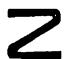
\includegraphics[keepaspectratio]{images/part002_ebb97593.jpg}}

